\documentclass[11pt]{exam}
%\documentclass[11pt,answers]{exam}

\usepackage[a4paper,margin=2cm]{geometry}
\parskip   2ex
\parsep    2ex
\itemsep   2ex
\parindent 0mm

\usepackage{graphicx}
\usepackage{color}
\usepackage{algorithm}
\usepackage{algorithmic}
\usepackage[tbtags]{amsmath}
\usepackage{amssymb}
\usepackage{amsfonts}
\usepackage{latexsym}
\usepackage{multirow}
\usepackage{hyperref}
\usepackage{cleveref}
\usepackage{subcaption}

\usepackage{listings}
% https://tex.stackexchange.com/a/17268
\lstset{
  literate={~} {$\sim$}{1},
  basicstyle=\ttfamily,
}

\pagestyle{empty}

\usepackage{filecontents}
\begin{filecontents}{\jobname.bib}
@Article{Miehe2014d,
  author    = {C. Miehe and F. E. Hildebrand and L. Boger},
  title     = {Mixed variational potentials and inherent symmetries of the Cahn-Hilliard theory of diffusive phase separation},
  journal   = {Proceedings of the Royal Society A: Mathematical, Physical and Engineering Sciences},
  year      = {2014},
  volume    = {470},
  number    = {2164},
  pages     = {20130641--20130641},
  month     = {feb},
  doi       = {10.1098/rspa.2013.0641},
  publisher = {The Royal Society},
  timestamp = {2018.03.12},
}
@Article{Miehe2014e,
  author    = {C. Miehe and S. Mauthe and H. Ulmer},
  title     = {Formulation and numerical exploitation of mixed variational principles for coupled problems of Cahn-Hilliard-type and standard diffusion in elastic solids},
  journal   = {International Journal for Numerical Methods in Engineering},
  year      = {2014},
  volume    = {99},
  number    = {10},
  pages     = {737--762},
  month     = {jun},
  doi       = {10.1002/nme.4700},
  publisher = {Wiley-Blackwell},
}
@Article{Kaessmair2016a,
  author    = {S. Kaessmair and P. Steinmann},
  title     = {Comparative computational analysis of the Cahn{\textendash}Hilliard equation with emphasis on C1 continuous methods},
  journal   = {Journal of Computational Physics},
  year      = {2016},
  volume    = {322},
  pages     = {783--803},
  month     = {oct},
  doi       = {10.1016/j.jcp.2016.07.005},
  publisher = {Elsevier {BV}},
}
@Article{Wodo2011a,
  author    = {O. Wodo and B. Ganapathysubramanian},
  title     = {Computationally efficient solution to the Cahn{\textendash}Hilliard equation: Adaptive implicit time schemes, mesh sensitivity analysis and the 3D isoperimetric problem},
  journal   = {Journal of Computational Physics},
  year      = {2011},
  volume    = {230},
  number    = {15},
  pages     = {6037--6060},
  month     = {jul},
  doi       = {10.1016/j.jcp.2011.04.012},
  publisher = {Elsevier {BV}},
}
}
\end{filecontents}
\usepackage[backend=bibtex]{biblatex}
\bibliography{\jobname.bib}

\newcommand{\makeheader}[3]{%
\setcounter{question}{0}
\begin{center}
{\sc Numerical Solution of PDEs Using the Finite Element Method}\vspace{2ex}\\
{\sc Exercise #1:\ \ \ #2}\vspace{2ex}\\
\begin{tabular*}{\textwidth}{ll @{\extracolsep{\fill}}r}
Jean-Paul Pelteret & (\url{jean-paul.pelteret@fau.de}) & \multirow{2}{*}{#3} \\
Luca Heltai & (\url{luca.heltai@sissa.it}) & \\
\end{tabular*}
\end{center}
}
\newcommand{\makeprojectheader}[2]{%
\begin{center}
{\sc Numerical Solution of PDEs Using the Finite Element Method}\vspace{2ex}\\
{\sc Project:\ \ \ #1}\vspace{2ex}\\
\begin{tabular*}{\textwidth}{ll @{\extracolsep{\fill}}r}
Jean-Paul Pelteret & (\url{jean-paul.pelteret@fau.de}) & \multirow{2}{*}{#2} \\
Luca Heltai & (\url{luca.heltai@sissa.it}) & \\
\end{tabular*}
\end{center}
}
\newcommand{\makeresources}[1]{%
\rule{\textwidth}{0.6mm}
\textbf{Some useful resources}\\[1.5ex]
%#1 \\
#1 \par
\rule{\textwidth}{0.6mm}
}

\newcommand{\FINISHME}[1]{\textcolor{red}{#1}}


\begin{document}

%% ===== EXERCISE 0: Setup ====
%
%\clearpage
%\makeheader{0}{Setting up the IDE}{19 March 2018}
%\makeresources{%
%\url{https://www.dealii.org/8.5.1/doxygen/deal.II/step_1.html} \\
%\url{https://www.dealii.org/8.5.1/doxygen/deal.II/step_49.html}
%}
%
%\begin{itemize}
%\item Edit the file \verb|~/.bashrc| to contain the line source \verb|/scratch/smr2909/enable.sh|. 
%You can use gedit \verb|~/.bashrc| to open an editor. 
%\item Close and re-open your terminal to activate the changes.
%\item Check that this worked by typing \verb|echo $DEAL_II_DIR|. 
% You should see\\\verb|/scratch/smr2909/deal.II/install| printed to the screen.
%\item Please note that inside \verb|/scratch/smr2909/| there are the following folders:
%\begin{itemize}
%\item \verb|labs/| -- a folder with exercise sheets and example programs
%\item \verb|bin/| and \verb|apps/| -- several programs (you shouldn't need to access them directly, because they will be imported into your \verb|PATH| automatically)
%\item \verb|libs/|, \verb|candi/|, \verb|candi-build| -- libraries deal.II depends on.
%\item \verb|deal.II| -- source, build, and installation of deal.II.
%\item \verb|deal.II/dealii/examples/| -- all tutorial programs.
%\end{itemize}
%\item To make a copy of \verb|step-1|, configure, compile, and run it:
%\begin{lstlisting}[language=bash]
%$ cp -r /scratch/smr2909/labs/lab01/step-1 ~/
%$ cd ~/step-1
%$ cmake .
%$ make
%$ ./step-1
%\end{lstlisting}
%\item  IDE: open \verb|Qt Creator|.
%\end{itemize}


% ===== EXERCISE 1: Triangulation ====


\clearpage
\makeheader{1}{Creating and manipulating \texttt{Triangulation}s}{19 March 2018}
\makeresources{%
\url{https://www.dealii.org/8.5.1/doxygen/deal.II/step_1.html} \\
\url{https://www.dealii.org/8.5.1/doxygen/deal.II/step_49.html}
}

\begin{questions}

\question Using \verb|step-1| as a base:

\begin{parts}
\part Compile and run this tutorial on the command line or inside a suitable IDE, and inspect at the output.
\part Create a helper function that takes a reference to a Triangulation and prints the following information: 
\begin{itemize}
\item number of levels
\item number of cells
\item number of active cells
\end{itemize}
Test this with all of your meshes.
\end{parts}

\question Modifying an existing meshing function
\begin{parts}
\part Comment out the \verb|.set_manifold(0, ...)| line in \verb|second_grid()|. What happens now?
\part Output mesh two as an svg file instead of eps. 
 Open it in a browser to display it (\verb|Firefox|, for example).
\part Go into \verb|second_grid()| and remove the last line (\verb|.set_manifold(0);|). The program will crash when you run it. 
Try to find out what is going on by debugging the program \hbox{(e.g. For \verb|Qt Creator|: ``Debug'' $\rightarrow$ ``Start debugging'')} and stepping through the function \linebreak\hbox{\verb|second_grid()|}. 
You can fix this problem in a more elegant way than putting the line you removed back in. 
How? See the tutorial description for more info.
\end{parts}

\question Creating a mesh from scratch
\begin{parts}
\part Generate a circle using \verb|GridGenerator::hyper_ball()| in 2d  (add a function \verb|third_grid()| to \verb|step-1|).
\begin{subparts}
\subpart Use a \verb|SphericalManifold| everywhere, only on the boundary, or on all cells except the center cell and refine the mesh globally twice.
\subpart  Set the output format of the previous example to \verb|vtk| and inspect the mesh in \verb|Paraview|.
\end{subparts}
\part Create an image of an L-shape domain with one global refinement.
\begin{subparts}
\subpart Inspect the mesh in \verb|Paraview|.
\subpart Refine the L-shaped mesh adaptively:
\begin{subsubparts}
\subsubpart Refine all cells with the distance between the center of the cell and re-entrant corner is smaller than $\frac{1}{3}$.
\subsubpart Refine exactly at the re-entrant corner (i.e. those with the corner as a vertex) several times.
\end{subsubparts}
\end{subparts}
\end{parts}

\question Reading in a mesh
\begin{parts}
\part Take a look at \verb|step-49| and read the included \verb|.msh| file in your modified \verb|step-1| program.
\part Add two levels of refinement to the cells at the boundary of the cut-outs.
\end{parts}

\question Additional tasks
\begin{parts}
%\bonuspart Create a regular grid; assign material IDs in checkerboard pattern; verify IDs
\bonuspart Create a mesh that represents the surface of a torus and refine it 2 times globally. Output to \verb|vtk| format and check the output. Note that your \verb|Triangulation| needs to be of type \verb|Triangulation<2,3>| (not explicitly discussed in this course).
\end{parts}

%\begin{solution}
%Meh
%\end{solution}

\end{questions}


% ===== EXERCISE 2: DoFHandler, DoFRenumbering, sparsity patterns ====


\clearpage
\makeheader{2}{Creating a \texttt{DoFHandler} and visualising sparsity patterns}{19 March 2018}
\makeresources{%
\url{https://www.dealii.org/8.5.1/doxygen/deal.II/step_2.html} \\
\url{https://www.dealii.org/8.5.1/doxygen/deal.II/namespaceDoFRenumbering.html}
}

\begin{questions}

\question Using \verb|step-2| as a base:
\begin{parts}
\part Compile and run this tutorial, and inspect at the output.
\part Look at the generated sparsity patterns (\verb|Firefox|, for example).
\end{parts}

\question Investigate:
\begin{parts}
\part How does the pattern change if you increase the polynomial degree from 1 to 2, or to 3?
\part \label{Ex 2: Refined unit square} How does the pattern change if you use a globally refined (say 3 times) unit square?
\part Are these patterns symmetric? Why/why not?
\part How many entries per row in the sparsity pattern do you expect for a \verb|Q1| element (assuming four cells are around each vertex)? 
\begin{subparts}
\subpart Check that this is true for the mesh in (\ref{Ex 2: Refined unit square}) (look for \verb|row_length(i)| and output them for each row). 
\subpart Can you construct a 2d mesh (without hanging nodes) that has a row with more entries?
\end{subparts}
\part How many entries per row in the sparsity pattern are there for \verb|Q2| and \verb|Q3| elements, again assuming four cells around each vertex?
\part Print all entries for row 42 for the original renumbered sparsity pattern.
\part Renumber the DoFs using the \verb|boost::king_ordering| algorithm. What does the sparsity pattern look like now?
\end{parts}

\question Additional tasks
\begin{parts}
\bonuspart Compute and output statistics like the number of unknowns, bandwidth of the sparsity pattern, average number of entries per row, and fill ratio.
\bonuspart Investigate the other appropriate DoF renumbering schemes. Which one produces the most banded structure?
\bonuspart Repeat the above for increasing refinement levels. Which is the most efficient scheme (lets say, in terms of bandwidth reduction versus computational time expended)?  You can get an estimate of the time for this operation like this:
\begin{lstlisting}[language=bash]
$ time ./step-2
\end{lstlisting}
\bonuspart What happens if you change the mesh from 2d to 3d?
\bonuspart Investigate the sparsity patterns generated for other types of \verb|FiniteElement|s of varying order.
\end{parts}

\end{questions}


% ===== EXERCISE 3: Poisson problem ====


\clearpage
\makeheader{3}{Solving the Poisson problem}{19 March 2018}
\makeresources{%
\url{https://www.dealii.org/8.5.1/doxygen/deal.II/step_3.html} \\
\url{https://www.dealii.org/8.5.1/doxygen/deal.II/step_4.html}
}

\begin{questions}

\question Using \verb|step-3| as a base:
\begin{parts}
\part Compile and run this tutorial, and inspect at the output.
\part Modify the code so that the problem is dimension-independent.
\part Switch to \verb|vtk| output and visualize in \verb|Paraview|. Figure out how to warp the solution by the solution variable.
\part Add a zero Neumann boundary condition to one edge of the domain.
%\begin{subparts}
Assign this Neumann boundary the indicator 1. \\
Tip: Look at the instructions in ``Modify the type of boundary condition'' in the ``Possibilities for extensions'' section of the tutorial.
%\end{subparts}
\part Add a non-zero Dirichlet boundary condition to one edge of the domain.
\begin{subparts}
\subpart Set the value to $-0.5$ for the boundary with \hbox{indicator 1}. \\
Tip: Look at the instructions in ``A slight variation of the last point'' in the ``Possibilities for extensions'' section of the tutorial.
\subpart Change the setup to have $f = 0$. Compare this result to that where $f$ is non-zero.
\end{subparts}
\end{parts}

%1. See documentation of step-4 at https://www.dealii.org/8.5.0/doxygen/deal.II/step_4.html
%2. Write a member function void mesh_info() that prints the following information about the triangula- tion to the screen: 1) number of active cells, 2) number of active/used vertices, lines, quads, hexs (only if appropriate for the dimension!).
%3. Use VectorTools::compute_mean_value (see step-3) and verify the convergence order of the mean in 2d and 3d.
%4. Gobacktostep-1andvisualizethesurfaceoftheTorusbycreatingaTriangulation<2,3>(2=dimension of the cells, 3=dimension of the space) using GridGenerator::torus if you haven’t done so.
%5. Try to use the function GridTools::rotate in make_grid() to rotate the mesh by 45 degrees (only in 2d!). Note that the function doesn’t exist in 3d (hint: function specialization).
%6. Change the mesh to an L-shape, only apply boundary values to the faces adjacent to the re-entrant corner (see set_boundary_indicator() in the step-3 description), change the boundary values to be 1 + ∥x∥2 and the right-hand side to be 1. Finally, visualize your solutions in ParaView in 2d and 3d.

\question Additional tasks
\begin{parts}
\bonuspart Do ``Convergence of the mean''. Can you see the order $h^{2}$? 
\bonuspart Increase the polynomial order (you need to increase all orders of the quadratures in the program!) and check the convergence of the mean now.
\bonuspart Switch to an L-shaped domain and experiment with a combination of Dirichlet and Neumann boundary conditions. 
By experimentation, identify the faces adjacent to the re-entrant corner and apply Dirichlet conditions only there. \\
Tip: There is more than one way to generate such a grid using the built-in functions. 
\end{parts}

\end{questions}

% ===== EXERCISE 4: Local (adaptive) refinement and computing errors ====


\clearpage
\makeheader{4}{Global and local error computation and estimation}{20 March 2018}
\makeresources{%
\url{https://www.dealii.org/8.5.1/doxygen/deal.II/step_6.html} \\
\url{https://www.dealii.org/8.5.1/doxygen/deal.II/step_7.html} \\
\url{https://www.dealii.org/8.5.1/doxygen/deal.II/group__numerics.html}
}

\begin{questions}

\question Using \verb|step-5| (or your previously modified version of \verb|step-3|) as a base:
\begin{parts}
\part \begin{align*}
-\Delta u(\mathbf{x}) &= f(\mathbf{x}) \quad \textnormal{in} \quad \Omega \in [0,1]^{2}, \quad \textnormal{with} \\
u(\mathbf{x}) &= \bar{u}(\mathbf{x})  \quad \textnormal{on} \quad \partial\Omega, \quad \textnormal{and} 
%\\
%f(\mathbf{x}) &= \begin{cases}
%1 &\quad \textnormal{if} \quad \vert xy \vert > 0.05 \\
%-1 &\quad \textnormal{otherwise}.
%\end{cases}
\end{align*}
\part Set the boundary conditions $\bar{u}(\mathbf{x})$ and forcing function $f(\mathbf{x})$ to get the manufactured solution
\begin{gather*}
u(\mathbf{x}) = \sin(\pi x_{1}) \; \cos(\pi x_{2}) .
\end{gather*}
Make sure the $\mathcal{L}^{2}$ errors are converging.\\
Tip: Look at the \verb|VectorTools::integrate_difference| function.
\part Implement the computation of the $\mathcal{H}^{1}$ error. \\
Tip: For this you need to compute and implement the gradient of the manufactured solution.
\part Use the \verb|KellyErrorEstimator| to predict where the regions of geometry where the solution approximation is inaccurate.
Visualise this error using \verb|Paraview|.
Do you observe any correlation between the gradient of the solution and the estimated local solution error? \\
Tip: Use a different quadrature rule to prevent super-convergent effects when using the \verb|KellyErrorEstimator|.
\part Perform local cell marking and refinement using the cell-based estimated error.
For this, the logic of the \verb|refine_mesh| function must be modified.
\end{parts}

\begin{solution}
Method of manufactured solutions:\\
See \url{http://www.personal.psu.edu/jhm/ME540/lectures/VandV/MMS_summary.pdf}
\begin{align*}
u(\mathbf{x}) 
 &= \sin(\pi x_{1}) \; \cos(\pi x_{2}) \\
\nabla u(\mathbf{x}) 
 &=\begin{bmatrix}
 \pi \cos(\pi x_{1}) \; \cos(\pi x_{2}) \\
 -\pi \sin(\pi x_{1}) \; \sin(\pi x_{2})
 \end{bmatrix} \\
\nabla \cdot \left[ \nabla u(\mathbf{x}) \right]
  = \Delta u(\mathbf{x})  
 &= -\pi^{2} \left[ \sin(\pi x_{1}) \; \cos(\pi x_{2}) + \sin(\pi x_{1}) \; \cos(\pi x_{2}) \right] \\
 &= -2\pi^{2} u(\mathbf{x}) 
\end{align*}
Therefore, we need to set 
\begin{align*}
\bar{u}(\mathbf{x}) &= \sin(\pi x_{1}) \; \cos(\pi x_{2}) \\
f(\mathbf{x}) &= -2\pi^{2} \bar{u}(\mathbf{x}) 
\end{align*}
\end{solution}

% Lab 5
%1. The topic of this lab session is a modified version of step-4 made available for you https://www.dealii. org/8.5.0/doxygen/deal.II/step_4.html
%2. For more information about computing errors see step-7 (it is a bit more complicated though) https: //www.dealii.org/8.5.0/doxygen/deal.II/step_7.html
%3. Run the program and check the graphical and text output.
%4. Where is the right-hand side defined and where do the boundary conditions come from?
%5. Fix the right-hand side and boundary conditions to get the manufactured solution
%u(x) = \sin(\pi x) · \cos(\pi y)
%and make sure the L2 errors are converging.
%6. Increase the polynomial degree of the finite element space and check the convergence of the L2 error.
%7. Implement the computation of the H1 error. For this you need to compute the gradient of the manufactured solution and implement it (see commented out code for a start).
%8. Implement a suitable 3d manufactured solution and test the convergence.

% Lab 7
%1. The topic of this lab session is a modified version of step-4 made available for you and the goal is to implement adaptive refinement based on step-6, see https://www.dealii.org/8.5.0/doxygen/deal.II/ step_6.html
%2. Modify the included program to support adaptive refinement by adding a ConstraintMatrix and the necessary function calls in setup (to create the constraints), assembly (distribute_local_to_global and no apply_boundary_values), solve (distribute), and replace the logic in refine_mesh.
%3. What happens if you “forget” the call constraints.distribute(solution) after solving the linear system?
%4. Use constraints.print (std::cout); to show the constraints if you have the following mesh in 2d:
%     GridGenerator::hyper_cube(triangulation);
%     triangulation.refine_global (1);
%     triangulation.begin_active()->set_refine_flag ();
%     triangulation.execute_coarsening_and_refinement ();
%and also look at this mesh (for example in paraview). Does the result make sense to you? Also compare with/without adding boundary conditions!
% 5. Change the problem to be an L-shape in 3d (start with 2 global refinements) and manufactured solution u(x, y, z) = 1 .
% r2 + 0.001
%Make sure you apply the correct right-hand side and boundary conditions.
%6. Compute the L2 error with respect to the number of DoFs with a) global refinement and b) adaptive refinement using a KellyEstimator like in step-6.
%7. Plot the two graphs in 4) in a log-log plot and include the line for a quadratic rate. Note that h2 =N−2/3.

\question Additional tasks
\begin{parts}
\bonuspart Compare the convergence rates (number of DoFs versus the solution error, best viewed in a log-log plot) when using global refinement and when using local refinement with the Kelly error estimator.
\bonuspart Investigate the influence of the coarsening and refinement parameters on the solution accuracy.
\bonuspart Investigate the effect of changing the polynomial order for the solution ansatz on the solution accuracy.
\bonuspart Integrate a non-constant coefficient into the governing equation, i.e. solve the heterogeneous Poisson equation
\begin{gather*}
-\alpha(\mathbf{x}) \Delta u(\mathbf{x}) = f(\mathbf{x}) \quad \textnormal{in} \quad \Omega
\end{gather*}
where $\alpha(\mathbf{x})$ represents some material parameter.
Repeat the calculation of the error using the \verb|KellyErrorEstimator|, while taking this spatially dependent coefficient into consideration. 
Tip: Look at the documentation for the \verb|KellyErrorEstimator| before deciding on how to implement $\alpha(\mathbf{x})$.
\bonuspart Choose $\alpha(\mathbf{x})$ to be spatially discontinuous.
Do you observe any correlation between the location of the material discontinuity and the estimated local solution error?
What influence does this have on the location of the refined cells?
Tip: Verify your conclusions by looking to the results of \verb|step-6|.
Further information can be found in the discussion ``Playing with the regularity of the solution'' in the ``Possibilities for extensions'' section of \verb|step-6|.
\end{parts}

\end{questions}


% ===== EXERCISE 5: Local refinement, hanging nodes and the ConstraintMatrix ====


\clearpage
\makeheader{5}{Local refinement, hanging nodes and the \texttt{ConstraintMatrix}}{20 March 2018}
\makeresources{%
\url{https://www.dealii.org/8.5.1/doxygen/deal.II/step_4.html} \\
\url{https://www.dealii.org/8.5.1/doxygen/deal.II/step_5.html} \\
\url{https://www.dealii.org/8.5.1/doxygen/deal.II/namespaceGridGenerator.html} \\
\url{https://www.dealii.org/8.5.1/doxygen/deal.II/namespaceVectorTools.html} \\
\url{https://www.dealii.org/8.5.1/doxygen/deal.II/namespaceDoFTools.html} \\
\url{https://www.dealii.org/8.5.1/doxygen/deal.II/group__constraints.html} \\
\url{https://www.dealii.org/8.5.1/doxygen/deal.II/step_49.html}
}

\begin{questions}

\question Using \verb|step-5| (or your previously modified version of \verb|step-3|) as a base:
\begin{parts}
\part Solve Laplace's equation
\begin{align*}
-\Delta u(\mathbf{x}) = 0 &\quad \textnormal{in} \quad \Omega, \quad \textnormal{with} \\
u(\mathbf{x}) = 0  &\quad \textnormal{on} \quad \partial\Omega_{1}, \quad \textnormal{and} \\
u(\mathbf{x}) = 1  &\quad \textnormal{on} \quad \partial\Omega_{2}
\end{align*}
on an L-shaped domain with length and width of dimension 1. Here, $\Omega_{2}$ denotes one of the end-edges of the L, and $\partial\Omega_{1} = \partial\Omega \backslash \partial\Omega_{2}$.
\part Starting from a coarse grid, perform successive global refinements to increase the accuracy of the solution and to locate the singularity.
\part \label{Ex 4: Hanging node constraints} Now switch from using global refinement to using local refinement in the vicinity of the singularity.
To accomplish this, you'll need to build the hanging node constraints. 
\part Build the Dirichlet boundary directly into a global \verb|ConstraintMatrix|, along with the existing hanging node constraints.
With this change, several parts of your code need to be modified:
\begin{subparts}
\subpart The constraints need to be built in the \verb|setup| function. \\
Tip: You can use the \verb|VectorTools::interpolate| function here.
\subpart The \verb|ConstraintMatrix| should be used to distribute local cell and vector contributions to their global counterparts.
\subpart The constraints must be distributed to the solution.
\end{subparts}
\end{parts}

\question Additional tasks
\begin{parts}
\bonuspart Following (\ref{Ex 4: Hanging node constraints}), what happens if you ``forget'' to distribute the (hanging node) constraints after solving the linear system?
\bonuspart Instead of using the \verb|VectorTools::interpolate| function, construct the Dirichlet contributions to the \verb|ConstraintMatrix| manually. \\
Tip: There are two ways to accomplish this: (1) Use the tools provided in the \verb|DoFTools| namespace, or (2) loop over cell faces and interrogate them for global DoFs that have support there.
\bonuspart Experiment with some of the other grids in the \verb|GridGenerator| namespace, such as \\\verb|GridGenerator::hyper_cross| and \verb|GridGenerator::cheese|, or create your own by using some of the grid modification tools discussed in \verb|step-49|.
In each case, find ways to efficiently increase the cell density in the location of singularities.
\bonuspart Using your existing code, replicate the study performed in \verb|step-5|. 
Note that the governing equation has changed slightly. 
Can you further improve the accuracy of the result in \verb|step-5| using Manifolds? \\
Tip: Look to the discussion ``A better mesh'' in the ``Possibilities for extensions'' section of \verb|step-6|.
\end{parts}

\end{questions}


% ===== EXERCISE 6: Shared memory parallelisation ====


\clearpage
\makeheader{6}{Shared memory parallelisation}{20 March 2018}
\makeresources{%
\url{https://www.dealii.org/8.5.1/doxygen/deal.II/step_6.html} \\
\url{https://dealii.org/8.5.1/doxygen/deal.II/group__threads.html} \\
\url{https://dealii.org/8.5.1/doxygen/deal.II/classThreads_1_1TaskGroup.html} \\
\url{https://www.dealii.org/8.5.1/doxygen/deal.II/namespaceWorkStream.html}
%\url{https://www.dealii.org/8.5.1/doxygen/deal.II/classFEValuesBase.html}
}

\begin{questions}

%\question \FINISHME{TaskGroup
%\begin{itemize}
%\item Note: Output using DataOut in tasks leads to seg fault (?) - get them to investigate this
%\item What else could they parallelise? Maybe get them to investigate this themselves?
%\begin{itemize}
%\item Assembly - would need to create a PerTaskData like struct per task
%\end{itemize}
%\end{itemize}
%}

\question Using \verb|step-6| or the outcome of the previous exercise as a base:
\begin{parts}
\part Parallelise the following parts of your code using \verb|TaskGroup| class:
\begin{subparts}
\subpart The system setup function.
Can you parallelise the two calls the fill the \verb|constraints|?
\subpart The assembly loop.
\subpart The (manual) calculation of the solution $\mathcal{L}^{2}$ norm.
\end{subparts}
\part Parallelise the following parts of your code using \verb|TBB| via the \verb|WorkStream| class:
\begin{subparts}
\subpart The assembly loop.
\subpart The (manual) calculation of the solution $\mathcal{L}^{2}$ norm.
\end{subparts}
\part Investigate the possible speed-up by playing around with the number of threads set in the call to \verb|Utilities::MPI::MPI_InitFinalize|. \\
Tip: This class needs to be created in the \verb|main| file before you create and execute your problem class.
\end{parts}

%- Assembly
%- Vector norm (chunks of a vector at a time)
%- Post-processing

\question Additional tasks
\begin{parts}
\bonuspart What influence do the \verb|queue_length| and \verb|chunk_size| have on the efficiency of the various parallel operations that you have implemented?
\bonuspart Perform some timings and compare the results:
\begin{subparts}
\subpart The serial version of this code.
\subpart The TBB threaded version of the code, but enforcing the use of one thread via the call to \verb|Utilities::MPI::MPI_InitFinalize|.
\subpart The TBB threaded version of the code using the maximum number of threads.
\end{subparts}
%\bonuspart Implement additional data post-processors, parallelise them, and visualise their output:
%\begin{subparts}
%\subpart The cell-wise material identifier.
%\subpart The cell-wise average solution $\frac{1}{V}\int_{\Omega^{K}} \phi \left(\mathbf{x}\right) \, dV$
%%\subpart The cell-wise solution $\mathcal{L}^{2}$ norm. % Note: This requires get_function_values() to be used.
%%\subpart The cell-wise solution error $\mathcal{L}^{2}$ norm.
%\end{subparts}
%Tip: All of these outputs can be stored in a regular \verb|Vector| of length equal to the number of cells in the triangulation.
\end{parts}

\end{questions}


% ===== EXERCISE 7: MPI parallelisation: Shared Triangulation ====


\clearpage
\makeheader{7 \& 8}{MPI parallelisation: \\\texttt{parallel::shared::Triangulation} and \texttt{parallel::distributed::Triangulation}}{21 March 2018}
\makeresources{%
\url{https://www.dealii.org/8.5.1/doxygen/deal.II/step_17.html} \\
\url{https://www.dealii.org/8.5.1/doxygen/deal.II/step_18.html} \\
\url{https://www.dealii.org/8.5.1/doxygen/deal.II/step_40.html} \\
\url{https://www.dealii.org/8.5.1/doxygen/deal.II/group__distributed.html} \\
\url{https://www.dealii.org/8.5.1/doxygen/deal.II/group__TrilinosWrappers.html} \\
\url{https://www.dealii.org/8.5.1/doxygen/deal.II/group__PETScWrappers.html}
}

% MpiInitFinalize
% pcout
% computing_timer
% Trilinos
% p::s::Tria
% IndexSet - locally owned, locally relevant
% Assembly; FilteredIterator
% Data output

% When do I need local data, i.e. KellyErrorEstimator

% RHS function: Rotated ellipse?
% Check the difference in performance between direct vs CG+AMG solver

% Additional question
% Would you need to add additional parallelisation (i.e. tbb) to the assembly loop. Why / why not? Under what conditions would this be beneficial?

% Lab 8
%1. Repeat the basic MPI commands from the file mpihello/main.cc
%2. Run the included step-40 using mpirun -n 4 ./step-40 and look at the graphical output.
%3. Similar to shown in lecture, visualize the view of the mesh from each individual processor using GridOut::write_svg and the “global” mesh. Use 3 MPI tasks for this.
%4. Now create a simple mesh (hyper_cube refined twice globally), run with two MPI tasks and print locally owned, locally active, and locally relevant IndexSet for each task.
%5. Switch to release mode (make release), decide on a global refinement level that takes in the order of 30-60 seconds to solve, and study assembly and solve time with 1,2,4,8,12,16 MPI tasks. Which is the fastest, do the timings make sense based on how many cores your machine has?
%6. Play with the test problem by switching to 3d and changing the geometry to something interesting. Your choice!

\begin{questions}

\question Using the supplied modified version of \verb|step-6| as a base:
\begin{parts}
\part For the first version of this code, use \verb|parallel::shared::Triangulation| and solve the 2d non-homogeneous Poisson equation 
\begin{align*}
- \alpha(\mathbf{x}) \Delta u(\mathbf{x}) &= f(\mathbf{x}) \quad \textnormal{in} \quad \Omega \in [0,1]^{2}, \quad \textnormal{with} \\
u(\mathbf{x}) &= 0  \quad \textnormal{on} \quad \partial\Omega,
\end{align*}
where
\begin{align*}
\alpha(\mathbf{x}) = \begin{cases}
5 &\quad \textnormal{if} \quad \vert \mathbf{x} - \mathbf{c} \vert < 0.2 \\
1 &\quad \textnormal{otherwise},
\end{cases}
\quad \textnormal{and} \quad
f(\mathbf{x}) = \begin{cases}
1 &\quad \textnormal{if} \quad \vert x_{1} x_{2} \vert > 0.05 \\
-10 &\quad \textnormal{otherwise},
\end{cases}
\end{align*}
and $\mathbf{c} = \left[0.6,0.6\right]^{T}$. 
The result similar to the following:  \\
\begin{figure}[!h]
\centering
\begin{subfigure}[t]{0.475\textwidth}
\centering
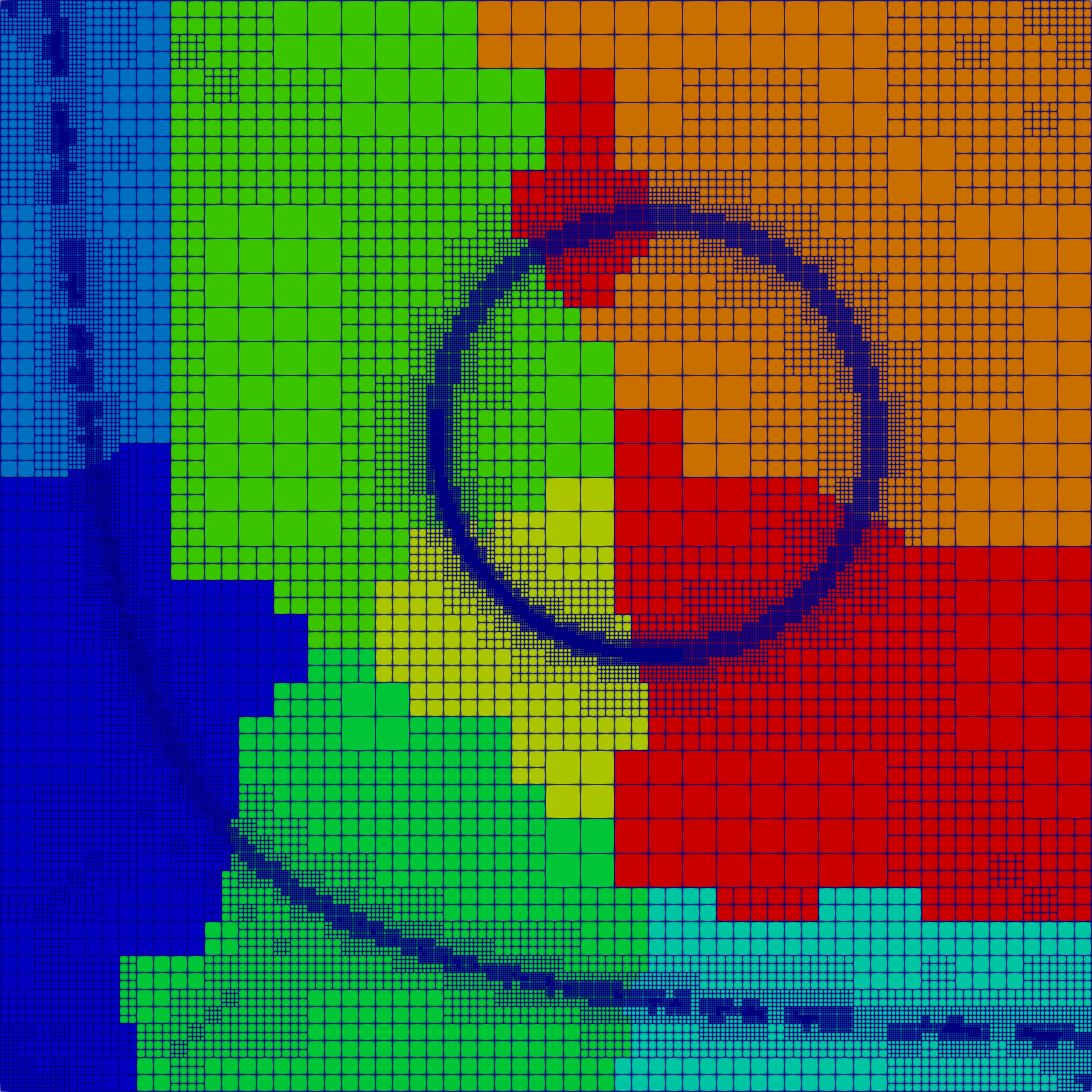
\includegraphics[height=0.225\textheight]{Figures/lab_07_08-partitioning.png}
\caption{Mesh and partitioning}
\end{subfigure}
\quad
\begin{subfigure}[t]{0.475\textwidth}
\centering
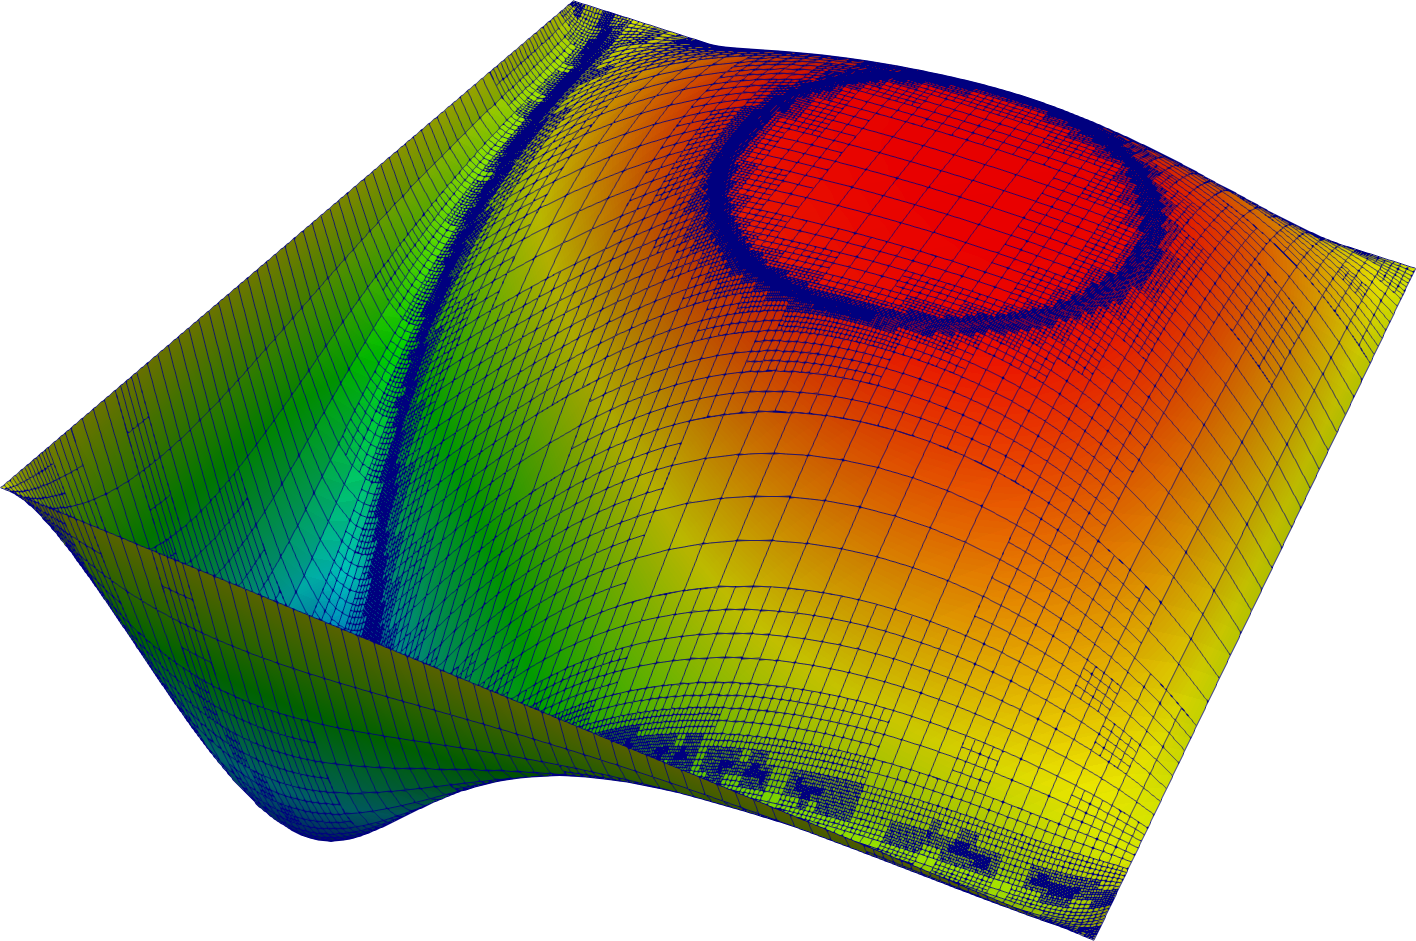
\includegraphics[height=0.225\textheight]{Figures/lab_07_08-solution.png}
\caption{Warped solution}
\end{subfigure}
\caption{Result produced from 3 initial global refinements and 8 refinement cycles, as visualised in \texttt{Paraview}.}
\end{figure}
\clearpage
These are the rough steps that you'll need to take to achieve this (look for the \verb|TODO|'s listed in the minimal code):
\begin{subparts}
\subpart Implement the functions defining the material coefficient $\alpha(\mathbf{x})$ and forcing function $f(\mathbf{x})$.
Extra credit for using a \verb|dealii::Function| for this purpose.
\subpart Initialise the MPI environment correctly in the \verb|main| function.
\subpart In the \verb|Step6| class constructor, initialise the class member variables correctly.
\subpart In the \verb|setup_system| function, initialise the sparsity pattern, system matrix, solution and RHS vectors correctly.
\subpart In the \verb|assemble_system| function:
\begin{subsubparts}
\subsubpart Configure the range of cells over which the assembly is performed.
\subsubpart Implement the forcing function.
\subsubpart Ensure synchronisation of the elements of the linear system at the end of the assembly loop.
\end{subsubparts}
\subpart In the \verb|solve| function, correctly choose the template parameter for the conjugate gradient solver, and select an appropriate preconditioner.
\subpart In the \verb|refine_grid| function, create the vector with entries required by the\\ \verb|KellyErrorEstimator|.
\subpart In the \verb|output_results| function, correctly construct the solution vector to be passed to \verb|DataOut| for later processing and visualisation.
\end{subparts}
\part Repeat the above using a \verb|parallel::distributed::Triangulation|.
\end{parts}

\question Additional tasks
\begin{parts}
\bonuspart Compare the distribution of cells across the processes for the two implementations. 
Is there a difference and, if so, why?
\bonuspart For this problem, measure the performance difference between the two implementations. 
What, do you think, are the primary factors affecting any differences you notice?
\bonuspart Investigate some of the various options for solvers (direct and iterative) and preconditioners.
For example, \verb|Trilinos| offers a direct solver, and its own implementation of iterative solvers, and numerous preconditioners.
Consider the properties of the linear system when deciding which options/combinations to test.
\bonuspart Similar to the previous task, investigate the use of \verb|PETSc| as the parallel linear algebra library.
%\bonuspart Investigate the use of the functions in the \verb|DerivativeApproximation| namespace as the refinement markers.
%Which is the most efficient option / combination for this problem when the 
\end{parts}

\end{questions}


%% ===== EXERCISE 8: MPI parallelisation: Distributed Triangulation ====
%
%
%\clearpage
%\makeheader{8}{MPI parallelisation: \texttt{parallel::distributed::Triangulation}}{21 March 2018}
%\makeresources{%
%\url{https://www.dealii.org/8.5.1/doxygen/deal.II/step_x.html}
%}
%
%\begin{questions}
%
%\question Using \verb|step-x| as a base:
%\begin{parts}
%\part x
%\end{parts}
%
%\question Additional tasks
%\begin{parts}
%\bonuspart x
%\end{parts}
%
%\end{questions}


%% ===== EXERCISE 9: ????? ====
%
%
%\clearpage
%\makeheader{9}{?????}{22 March 2018}
%\makeresources{%
%\url{https://www.dealii.org/8.5.1/doxygen/deal.II/step_x.html} \\
%\url{https://www.dealii.org/8.5.1/doxygen/deal.II/classParameterHandler.html} \\
%\url{https://www.dealii.org/developer/doxygen/deal.II/classParameterAcceptor.html} \\
%\url{https://www.dealii.org/8.5.1/doxygen/deal.II/group__LAOperators.html}
%}
%
%\begin{questions}
%
%\question \FINISHME{Possible exercise outline?}
%\FINISHME{
%\begin{itemize}
%\item Use Git to manage this project
%  \begin{itemize}
%  \item \url{https://github.com/dealii/dealii/wiki/Contributing}
%  \item Start at a previous step
%  \item Commit this to master
%  \item Create a new branch and work off of enhancements there
%  \end{itemize}
%\item Extend example to use ParameterHandler
%  \begin{itemize}
%  \item Constant coefficient for two material zones (heterogenous Poisson)
%  \item Function parser for RHS function / boundary conditions
%  \item Solver (iterative + direct)
%  \item Preconditioner
%  \item Tolerances
%  \end{itemize}
%\item Use linear operator:
%  \begin{itemize}
%  \item Solve initial problem using normal linear operators
%  \item Next, solve problem using constrained linear operator
%  \end{itemize}
%\item Add some doxygen documentation?
%\end{itemize}
%}
%
%\question Using \verb|step-x| as a base:
%\begin{parts}
%\part x
%\end{parts}
%
%\question Additional tasks
%\begin{parts}
%\bonuspart x
%\end{parts}
%
%\end{questions}
%
%
%% ===== EXERCISE 10: Time dependent problems and SolutionTransfer ====
%
%
%\clearpage
%\makeheader{10}{Time dependent problems and \texttt{SolutionTransfer}}{22 March 2018}
%\makeresources{%
%\url{https://www.dealii.org/8.5.1/doxygen/deal.II/step_23.html} \\
%\url{https://www.dealii.org/8.5.1/doxygen/deal.II/step_24.html} \\
%\url{https://www.dealii.org/8.5.1/doxygen/deal.II/group__LAOperators.html} \\
%\url{https://www.dealii.org/8.5.1/doxygen/deal.II/group__constraints.html} \\
%\url{https://www.dealii.org/8.5.1/doxygen/deal.II/namespaceTimeStepping.html}
%%\url{https://en.wikipedia.org/wiki/Potential_flow\#Sound_waves}
%%\url{https://en.wikipedia.org/wiki/Courant%E2%80%93Friedrichs%E2%80%93Lewy_condition}
%%https://www.dealii.org/developer/doxygen/deal.II/step_52.html
%}
%
%\begin{questions}
%
%\question Using \verb|step-23| as a base (or through appropriate modification of \verb|step-6|) we will be working through the ``Possibilities for extensions'' listed for \verb|step-23|.
%\begin{parts}
%\part The governing equations for the wave equation are
%\begin{align*}
%\frac{\partial^{2} u(\mathbf{x})}{\partial t^{2}} - u(\mathbf{x}) = f(\mathbf{x})  &\quad \textnormal{in} \quad \Omega \in [0,1]^{2} \times [0, T], \quad \textnormal{with} \\
%u(\mathbf{x},t) = \bar{u}(\mathbf{x}) = 0  &\quad \textnormal{on} \quad \partial\Omega
%\intertext{with initial conditions}
%u(\mathbf{x},0) = u_{0}(\mathbf{x})  &\quad \textnormal{in} \quad \Omega, \quad \textnormal{and} \\
%\frac{\partial u(\mathbf{x},0)}{\partial t} = u_{1}(\mathbf{x})  &\quad \textnormal{in} \quad \Omega.
%\end{align*}
%\part Build the boundary conditions into a \verb|ConstraintMatrix|, instead of using \\\verb|MatrixTools::apply_boundary_values|.
%\part Rewrite the linear system solution scheme in the \verb|run| function using the \verb|linear_operator| and  \verb|constrained_linear_operator| class construction functions. (Note: The latter helps prevent having to reconstruct the solution-independent matrices $\mathbf{M}$ and $\mathbf{A}$ at each timestep).
%\part Use \verb|Sundials| to do time integration. Use \verb|Sundials::ARKode| (full implicit, full explicit, semi-implicit).
%\begin{subparts}
%\subpart Minimum: Reinit vector, implicit or explicit functions
%\subpart Solve jacobian system
%\end{subparts}
%\part Implement adaptive mesh refinement using the \verb|KellyErrorEstimator|, refining and coarsening the mesh after every $n$-timesteps.
%You now need to consider the discussion in the last point of ``Possibilities for extensions''.
%Basically, during the refinement process you will need to interpolate the solution stored for the previous timestep onto the new mesh; this task can be accomplished using the \verb|SolutionTransfer| class. \\
%Tip: Take special care when dealing with hanging nodes!
%\part Consider the governing equation with non-homogeneous coefficients
%\begin{gather}
%\rho(\mathbf{x}) \frac{\partial^{2} u(\mathbf{x})}{\partial t^{2}} - \alpha(\mathbf{x}) u(\mathbf{x}) = f(\mathbf{x})
%\end{gather}
%where $t$ denotes the time, $\rho$ the material density and $\alpha$ its stiffness modulus.
%How would you implement a time stepping scheme that better ensures that the CFL condition, namely that
%\begin{gather*}
%\Delta t \leq \frac{h}{c} \quad \textnormal{with} \quad c = \sqrt{\frac{\alpha}{\rho}} \quad ?
%\end{gather*}
%You may look to \verb|step-24|, in particular the discussion in the \verb|setup_system| section, for some tips.
%\end{parts} 
%
%\question Additional tasks
%\begin{parts}
%\bonuspart Investigate the role of the time stepping parameter $\theta$, used as part of the fractional step method.
%\bonuspart Rewrite the timestepping scheme making use of the \verb|TimeStepping| class. An example of the use of \verb|RungeKutta| methods is given in \href{https://www.dealii.org/developer/doxygen/deal.II/step_52.html}{\texttt{step-52}}.
%\end{parts}
%
%\end{questions}
%
%
%% ===== EXERCISE 11: Automatic differentiation using Sacado ====
%
%
%\clearpage
%\makeheader{11}{Automatic differentiation using Sacado}{22 March 2018}
%\makeresources{%
%\url{https://www.dealii.org/8.5.1/doxygen/deal.II/step_6.html}\\
%deal.II test-suite: \\
%\url{https://github.com/dealii/dealii/blob/master/tests/sacado/basic_01.cc}\\
%\url{https://github.com/dealii/dealii/blob/master/tests/sacado/basic_01a.cc}\\
%\url{https://github.com/dealii/dealii/blob/master/tests/sacado/basic_01b.cc}\\
%\url{https://github.com/dealii/dealii/blob/master/tests/sacado/basic_02.cc}\\
%\url{https://github.com/dealii/dealii/blob/master/tests/sacado/basic_02a.cc}\\
%\url{https://github.com/dealii/dealii/blob/master/tests/sacado/basic_02b.cc}
%}
%
%\begin{questions}
%
%\question \label{Ex 11: AD scalar functions} Compute the stipulated derivatives of the following functions using the \verb|Sacado::Fad::DFad| auto-differentiable number type. Verify your results.
%\begin{parts}
%\part \FINISHME{First derivatives only}
%\begin{subparts}
%\subpart $f(x) = \exp(2x)\ln(-2x)$ evaluated at $x = \frac{7\pi}{17}$.
%\begin{solution}
%% WolframAlpha: derivative of exp(2x)*ln(-2x)
%$\frac{\exp{(2 x)} (2 \ln(-2 x) + 1)}{x}$
%\end{solution}
%\subpart $f(x,y) = \sin(x^2-xy)$ evaluated at $x = $, $y = $
%\begin{solution}
%% mAlpha: derivative of sin(x*x - x*y) wrt x
%$(2 x - y) \cos(x (x - y))$
%% WolframAlpha: derivative of sin(x*x - x*y) wrt y
%$-x \cos(x (x - y))$
%\end{solution}
%\end{subparts}
%\part \FINISHME{First and second derivatives}
%\begin{subparts}
%\subpart $f(x) = $ evaluated at $x = $.
%\subpart $f(x,y) = $ evaluated at $x = $, $y = $.
%\end{subparts}
%\end{parts}
%
%
%\question \label{Ex 11: AD FEM} Using \verb|step-x| as a base:
%\begin{parts}
%\part Using the nested \verb|Sacado::Fad::DFad| auto-differentiable number type, solve Laplace's equation
%\begin{align*}
%-\Delta u(\mathbf{x}) = 0 &\quad \textnormal{in} \quad \Omega \in [0,1]^{2}, \quad \textnormal{with} \\
%u(\mathbf{x}) = 0  &\quad \textnormal{on} \quad \partial\Omega_{1}, \quad \textnormal{and} \\
%u(\mathbf{x}) = 1  &\quad \textnormal{on} \quad \partial\Omega_{2}
%\end{align*}
%on an L-shaped domain with length and width of dimension 1. Here, $\Omega_{2}$ denotes one of the end-edges of the L, and $\partial\Omega_{1} = \partial\Omega \backslash \partial\Omega_{2}$.   \\
%Tip: For this linear problem, you'll need to consider the energy functional
%\begin{gather*}
%\Pi = \frac{1}{2}\int_{\Omega} \nabla u \cdot \nabla u \; \textnormal{dV} 
%\quad \rightarrow \quad \textnormal{min}.
%\end{gather*}
%\part Extend the above to include the forcing function  
%% WolframAlpha: plot 0.5*cos(5*pi*x*y)+0.5 for x=0..1, y=0..1
%\begin{gather*}
%f(\mathbf{x}) = \begin{cases}
%1 &\quad \textnormal{if} \quad \frac{1}{2}\cos(5\pi x_{1} x_{2})+0.5 > 0.5 \\
%0 &\quad \textnormal{otherwise}.
%\end{cases}
%\end{gather*}
%Tip 1: For this linear problem, you'll need to consider the energy functional
%\begin{gather*}
%\Pi = \frac{1}{2}\int_{\Omega} \nabla u \cdot \nabla u \; \textnormal{dV}
%    + \int_{\Omega} u \cdot f \; \textnormal{dV}
%\quad \rightarrow \quad \textnormal{min}.
%\end{gather*}
%%\FINISHME{Can this be done like this, or does one need to add the traction separately?\\}
%Tip 2: You will also need to recall the finite element discretisation for the solution
%\begin{gather*}
%u (\mathbf{x}) = \sum_{I} N^{I} (\mathbf{x}) \; u^{I}
%\end{gather*}
%where $N^{I}$ is the shape function associated with the $I^{th}$ degree-of-freedom, and $u^{I}$ are solution coefficients.
%\end{parts}
%
%\question Additional tasks
%\begin{parts}
%\bonuspart Following up on \ref{Ex 11: AD scalar functions}, try to write a simple nonlinear solution scheme using \verb|Sacado::Fad::DFad| to solve for the roots of $f(x) = 5x^3 + 3x + 1$.
%\bonuspart Following up on \ref{Ex 11: AD FEM}, can you achieve the same goal using a nested\\ \verb|Sacado::Rad::ADvar<Sacado::Fad::DFad>|? How does the performance of this implementation compare to that of the \verb|Sacado::Fad::DFad<Sacado::Fad::DFad>|?
%\end{parts}
%
%\end{questions}
%
%
%% ===== Project ====
%
%
%\clearpage
%\makeprojectheader{Implementing the Cahn-Hiliard equations}{23 March 2018}
%%\url{https://www.dealii.org/8.5.1/doxygen/deal.II/step_x.html}
%%\leavevmode
%\makeresources{%
%\vspace*{-3\parsep}
%\begin{enumerate}
%\item \fullcite{Miehe2014d}
%\item \fullcite{Miehe2014e}
%\item \fullcite{Kaessmair2016a}
%\item \fullcite{Wodo2011a}
%\end{enumerate}%
%\vspace*{-\parsep}
%}
%\begin{questions}
%
%\question \FINISHME{Finish this}
%\FINISHME{
%\begin{itemize}
%\item Implement a solution to the Cahn-Hiliard equation
%\begin{itemize}
%\item Implementation based on Miehe paper
%\item Scalar (non-coupled) time dependent problem.
%\item Is it possible to implement other time stepping schemes? Miehe explicity uses backward Euler
%\item We have a base solution for the elastic-coupled problem, courtesy of S. Kaessmair which we can use to validate the student's work (we should attribute him on the tutorial as well).
%\item Timestepping: 
%\item Starting concentration: !=0.5 (0.5 leads to a bubble)
%\end{itemize}
%\item Parallelisation using MPI
%\item Assembly using automatic differentiation (Sacado)
%\begin{itemize}
%\item Start with formulation based on energy functional (twice differentiated)
%\item Next do residual-based formulation (one differentiated)
%\item Lastly, do full manual linearisation
%\end{itemize}
%\item Local adaptivity
%\begin{itemize}
%\item Ensuring conservation properties is important, as the solution can get stuck in a local equilibrium (e.g. parallel bands of concentrated material)
%\item Refinement strategy around regions of high concentration gradient. Manual refinement strategy vs using e.g. Kelly error estimator. Need at least 4 cells in the band of changing concentration.
%\item Solution transfer; implications for time-stepping algorithm
%\end{itemize}
%\item Consolidate everything learned in the course
%\item Add this as a tutorial to the deal.II library
%\item Open a pull-request on Github
%\end{itemize}
%}
%
%\question Using \verb|step-x| as a base:
%\begin{parts}
%\part x
%\end{parts}
%
%\question Additional tasks
%\begin{parts}
%\bonuspart x
%\end{parts}
%
%\end{questions}

\end{document}